\documentclass[12pt]{article}
\setlength{\parindent}{0pt}

%%%%%%%%%%%%%%%%%%%%%%%%%%%%%%%%%%%%%%%%%%%%%%%%%%%%%%%%%%%%%%%%%%%%
% PAQUETES
%%%%%%%%%%%%%%%%%%%%%%%%%%%%%%%%%%%%%%%%%%%%%%%%%%%%%%%%%%%%%%%%%%%%
\usepackage[left=3cm, right=3cm, top=2.5cm, bottom=2.5cm]{geometry}
\usepackage{graphicx}
\usepackage{amsmath}
\usepackage{longtable}
\usepackage{subcaption}
\usepackage{booktabs}
\usepackage{enumitem}
\usepackage[hidelinks]{hyperref}
\usepackage[english]{babel}
\usepackage{csquotes}
\usepackage{tikz}
\usetikzlibrary{positioning, arrows.meta}
\usepackage{caption}
\usepackage{booktabs}
\usepackage{float}
\usepackage[
    backend=biber,
    style=apa,
    sorting=none
]{biblatex}
\addbibresource{references.bib}
\usepackage[font=footnotesize]{caption}

%%%%%%%%%%%%%%%%%%%%%%%%%%%%%%%%%%%%%%%%%%%%%%%%%%%%%%%%%%%%%%%%%%%%
% INICIO DOCUMENTO
%%%%%%%%%%%%%%%%%%%%%%%%%%%%%%%%%%%%%%%%%%%%%%%%%%%%%%%%%%%%%%%%%%%%
\begin{document}
%%%%%%%%%%%%%%%%%%%%%%%%%%%%%%%%%%%%%%%%%%%%%%%%%%%%%%%%%%%%%%%%%%%%
% PORTADA
%%%%%%%%%%%%%%%%%%%%%%%%%%%%%%%%%%%%%%%%%%%%%%%%%%%%%%%%%%%%%%%%%%%%
\begin{titlepage}
    \begin{center}
        \textbf{\Huge{Lakehouse Map of a 3-Tier Lakehouse for Mobility Data Analysis}}\\
        \vspace{400pt}
        Borja Albert Gramaje \& Joan Fernández Navarro
    \end{center}

    \hrule 
    \vspace{-5pt}
        \begin{center}
    	\Large{
            B\hspace{4pt}I\hspace{4pt}G\hspace{12pt}            D\hspace{4pt}A\hspace{4pt}T\hspace{4pt}A\\          E\hspace{4pt}N\hspace{4pt}G\hspace{4pt}I\hspace{4pt}N\hspace{4pt}E\hspace{4pt}E\hspace{4pt}R\hspace{4pt}I\hspace{4pt}N\hspace{4pt}G\hspace{12pt}            A\hspace{4pt}N\hspace{4pt}D\hspace{12pt}            T\hspace{4pt}E\hspace{4pt}C\hspace{4pt}H\hspace{4pt}N\hspace{4pt}O\hspace{4pt}L\hspace{4pt}O\hspace{4pt}G\hspace{4pt}I\hspace{4pt}E\hspace{4pt}S
        }\\
        \vspace{5pt}
        \normalsize{
            Master's Degree in Computational Engineering and Industrial Mathematics
        }
    \end{center}
    \vspace{-5pt}
    \hrule
    \vspace{20pt}
    \begin{figure}[h] 
		\flushright
        \includegraphics[height=0.1\linewidth]{images/upv-logo.jpg}
    \end{figure}
\end{titlepage}

\pagebreak
%%%%%%%%%%%%%%%%%%%%%%%%%%%%%%%%%%%%%%%%%%%%%%%%%%%%%%%%%%%%%%%%%%%%
% Lakehouse Map
%%%%%%%%%%%%%%%%%%%%%%%%%%%%%%%%%%%%%%%%%%%%%%%%%%%%%%%%%%%%%%%%%%%%
\section{Lakehouse Map}

\begin{figure}[H]
    \centering
    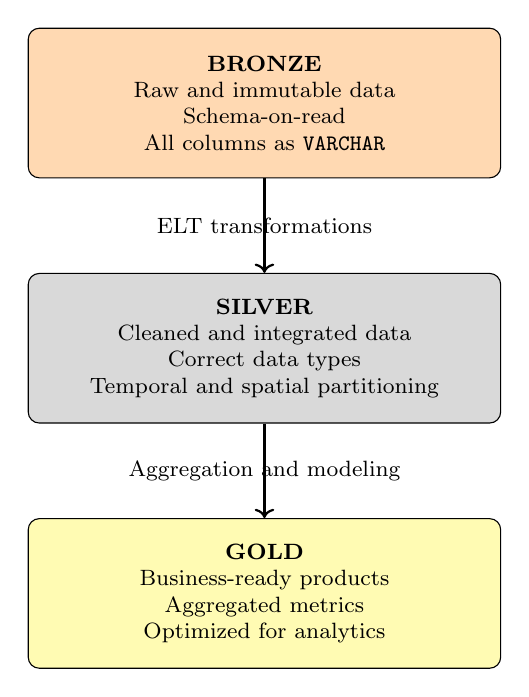
\begin{tikzpicture}[
        layer/.style={
            rectangle,
            draw,
            rounded corners,
            minimum width=6cm,
            minimum height=1.9cm,
            align=center,
            font=\footnotesize
        },
        arrow/.style={
            ->,
            thick
        }
    ]
    
    % Layers (top to bottom)
    \node[layer, fill=orange!30] (bronze) {
        \textbf{BRONZE}\\
        Raw and immutable data\\
        Schema-on-read\\
        All columns as \texttt{VARCHAR}
    };
    
    \node[layer, fill=gray!30, below=1.2cm of bronze] (silver) {
        \textbf{SILVER}\\
        Cleaned and integrated data\\
        Correct data types\\
        Temporal and spatial partitioning
    };
    
    \node[layer, fill=yellow!30, below=1.2cm of silver] (gold) {
        \textbf{GOLD}\\
        Business-ready products\\
        Aggregated metrics\\
        Optimized for analytics
    };
    
    % Arrows
    \draw[arrow] (bronze) -- node {\footnotesize ELT transformations} (silver);
    \draw[arrow] (silver) -- node {\footnotesize Aggregation and modeling} (gold);
    
    \end{tikzpicture}
    \caption{Three-tier lakehouse data pipeline.}
\end{figure}


\subsection*{Bronze Layer}
\begin{figure}[H]
    \centering
    \includegraphics[width=\linewidth]{images/bronze_diagram.png}
    \caption{Bronze layer schema representing the raw ingestion of mobility and demographic data.}
    \label{fig:placeholder}
\end{figure}

\subsection*{Silver Layer}
\begin{figure}[H]
    \centering
    \includegraphics[width=\linewidth]{images/silver_diagram.png}
    \caption{Silver layer schema showing cleaned, standardized, and integrated datasets.}
    \label{fig:placeholder}
\end{figure}

\subsection*{Gold Layer}
\begin{figure}[H]
    \centering
    \includegraphics[width=\linewidth]{images/gold_diagram.png}
    \caption{Gold layer schema illustrating business-ready analytical data products.}
    \label{fig:gold_schema}
\end{figure}
\pagebreak

%%%%%%%%%%%%%%%%%%%%%%%%%%%%%%%%%%%%%%%%%%%%%%%%%%%%%%%%%%%%%%%%%%%%
% Lakehouse Map
%%%%%%%%%%%%%%%%%%%%%%%%%%%%%%%%%%%%%%%%%%%%%%%%%%%%%%%%%%%%%%%%%%%%
\section{Data Sheets}

\section*{Bronze Layer}

\subsection*{Data Sheet: \texttt{bronze\_mitma\_od\_municipios}}
\begin{itemize}
    \item \textbf{Description:} Raw origin-destination mobility matrices by municipality, date, and hour from MITMA RSS feeds.
    \item \textbf{Grain:} One row per origin zone, destination zone, date, hour, and demographic segment.
    \item \textbf{Sources:} MITMA Estudios Básicos RSS feeds
    \item \textbf{Tracking:} \texttt{source\_file} column contains URL of source CSV file
\end{itemize}

\begin{longtable}{p{3cm} p{2cm} p{1.5cm} p{1.8cm} p{6cm}}
    \caption{Technical Data Sheet for the bronze\_mitma\_od\_municipios Table} \\
    \toprule
    \textbf{Column} & \textbf{Type} & \textbf{Unit} & \textbf{Nullable} & \textbf{Description} \\
    \midrule
    fecha & TIMESTAMP & -- & No & Date (parsed from YYYYMMDD format in source CSV)\\
    periodo & VARCHAR & -- & Yes & Hour of day (0-23)\\
    origen & VARCHAR & -- & No & Origin zone identifier\\
    destino & VARCHAR & -- & No & Destination zone identifier\\
    viajes & VARCHAR & trips & No & Number of trips (as string)\\
    viajes\_km & VARCHAR & trip-km & No & Total distance traveled (as string)\\
    distancia & VARCHAR & km & Yes & Distance category or band\\
    residencia & VARCHAR & -- & Yes & Residence classification\\
    source\_file & VARCHAR & -- & No & URL of source CSV file\\
    loaded\_at & TIMESTAMP & -- & No & Timestamp of ingestion\\
    \bottomrule
\end{longtable}
\pagebreak

\subsection*{Data Sheet: \texttt{bronze\_mitma\_municipios}}
\begin{itemize}
    \item \textbf{Description:} Raw zoning reference data including geometric boundaries for municipalities.
    \item \textbf{Grain:} One row per spatial zone.
    \item \textbf{Sources:} MITMA zoning shapefile exports
    \item \textbf{Tracking:} Single ingestion, no source\_file column
\end{itemize}

\begin{longtable}{p{3cm} p{2.5cm} p{1.8cm} p{7cm}}
    \caption{Technical Data Sheet for the bronze\_mitma\_municipios Table} \\
    \toprule
    \textbf{Column} & \textbf{Type} & \textbf{Nullable} & \textbf{Description}\\
    \midrule
    ID & VARCHAR & No & Unique spatial zone identifier\\
    Nombre & VARCHAR & No & Human-readable zone name\\
    geometry & VARCHAR & No & WKT (Well-Known Text) representation of polygon geometry\\
    loaded\_at & TIMESTAMP & No & Timestamp of ingestion\\
    \bottomrule
\end{longtable}
\pagebreak

\subsection*{Data Sheet: \texttt{bronze\_ine\_municipios}}
\begin{itemize}
    \item \textbf{Description:} Catalog of Spanish municipalities with INE codes and names from INE API.
    \item \textbf{Grain:} One row per municipality.
    \item \textbf{Sources:} INE API (JSON format)
    \item \textbf{Tracking:} \texttt{source\_url} column contains API endpoint URL
\end{itemize}

\begin{longtable}{p{3cm} p{2.5cm} p{1.8cm} p{7cm}}
    \caption{Technical Data Sheet for the bronze\_ine\_municipios Table} \\
    \toprule
    \textbf{Column} & \textbf{Type} & \textbf{Nullable} & \textbf{Description}\\
    \midrule
    Id & VARCHAR & No & INE internal identifier\\
    Codigo & VARCHAR & No & INE municipality code\\
    Nombre & VARCHAR & No & Municipality name\\
    source\_url & VARCHAR & No & INE API endpoint URL\\
    loaded\_at & TIMESTAMP & No & Timestamp of ingestion\\
    \bottomrule
\end{longtable}
\pagebreak

\subsection*{Data Sheet: \texttt{bronze\_ine\_empresas\_municipio}}
\begin{itemize}
    \item \textbf{Description:} Number of registered companies per municipality and year from INE API.
    \item \textbf{Grain:} One row per municipality and year (nested JSON structure).
    \item \textbf{Sources:} INE API (JSON format with nested Data array)
    \item \textbf{Tracking:} \texttt{source\_url} column contains API endpoint URL with year parameter
\end{itemize}

\begin{longtable}{p{3cm} p{2cm} p{1.5cm} p{1.8cm} p{6cm}}
    \caption{Technical Data Sheet for the bronze\_ine\_empresas\_municipio Table} \\
    \toprule
    \textbf{Column} & \textbf{Type} & \textbf{Unit} & \textbf{Nullable} & \textbf{Description} \\
    \midrule
    Codigo & VARCHAR & -- & No & INE municipality code\\
    Nombre & VARCHAR & -- & No & Municipality name\\
    Data & VARCHAR & -- & No & JSON array string containing year-value pairs\\
    source\_url & VARCHAR & -- & No & INE API endpoint URL\\
    loaded\_at & TIMESTAMP & -- & No & Timestamp of ingestion\\
    \bottomrule
\end{longtable}
\pagebreak

\subsection*{Data Sheet: \texttt{bronze\_ine\_poblacion\_municipio}}
\begin{itemize}
    \item \textbf{Description:} Population counts by municipality, sex, and year from INE API.
    \item \textbf{Grain:} One row per municipality and year (nested JSON structure).
    \item \textbf{Sources:} INE API (JSON format with nested Data array)
    \item \textbf{Tracking:} \texttt{source\_url} column contains API endpoint URL with year parameter
\end{itemize}

\begin{longtable}{p{3cm} p{2cm} p{1.5cm} p{1.8cm} p{6cm}}
    \caption{Technical Data Sheet for the bronze\_ine\_poblacion\_municipio Table} \\
    \toprule
    \textbf{Column} & \textbf{Type} & \textbf{Unit} & \textbf{Nullable} & \textbf{Description} \\
    \midrule
    Codigo & VARCHAR & -- & No & INE municipality code\\
    Nombre & VARCHAR & -- & No & Municipality name\\
    Data & VARCHAR & -- & No & JSON array string containing year-sex-value tuples\\
    source\_url & VARCHAR & -- & No & INE API endpoint URL\\
    loaded\_at & TIMESTAMP & -- & No & Timestamp of ingestion\\
    \bottomrule
\end{longtable}
\pagebreak

\subsection*{Data Sheet: \texttt{bronze\_ine\_renta\_municipio}}
\begin{itemize}
    \item \textbf{Description:} Average income per capita by municipality and year from INE API.
    \item \textbf{Grain:} One row per municipality and year (nested JSON structure).
    \item \textbf{Sources:} INE API (JSON format with nested Data array)
    \item \textbf{Tracking:} \texttt{source\_url} column contains API endpoint URL with year parameter
\end{itemize}

\begin{longtable}{p{3cm} p{2cm} p{1.5cm} p{1.8cm} p{6cm}}
    \caption{Technical Data Sheet for the bronze\_ine\_renta\_municipio Table} \\
    \toprule
    \textbf{Column} & \textbf{Type} & \textbf{Unit} & \textbf{Nullable} & \textbf{Description} \\
    \midrule
    Codigo & VARCHAR & -- & No & INE municipality code\\
    Nombre & VARCHAR & -- & No & Municipality name\\
    Data & VARCHAR & -- & No & JSON array string containing year-value pairs\\
    source\_url & VARCHAR & -- & No & INE API endpoint URL\\
    loaded\_at & TIMESTAMP & -- & No & Timestamp of ingestion\\
    \bottomrule
\end{longtable}
\pagebreak

\subsection*{Data Sheet: \texttt{bronze\_mitma\_ine\_relations}}
\begin{itemize}
    \item \textbf{Description:} Mapping table connecting MITMA zone identifiers to INE municipality codes.
    \item \textbf{Grain:} One row per MITMA-INE relationship.
    \item \textbf{Sources:} MITMA CSV file from movilidad-opendata.mitma.es
    \item \textbf{Tracking:} \texttt{source\_file} column contains source CSV URL
\end{itemize}

\begin{longtable}{p{3cm} p{2.5cm} p{1.8cm} p{7cm}}
    \caption{Technical Data Sheet for the bronze\_mitma\_ine\_relations Table} \\
    \toprule
    \textbf{Column} & \textbf{Type} & \textbf{Nullable} & \textbf{Description}\\
    \midrule
    municipio\_mitma & VARCHAR & No & MITMA zone identifier\\
    municipio\_ine & VARCHAR & No & INE municipality code\\
    source\_file & VARCHAR & No & Source CSV file URL\\
    loaded\_at & TIMESTAMP & No & Timestamp of ingestion\\
    \bottomrule
\end{longtable}
\pagebreak

\subsection*{Data Sheet: \texttt{bronze\_spanish\_holidays}}
\begin{itemize}
    \item \textbf{Description:} National holidays for Spain generated programmatically using Python's holidays library.
    \item \textbf{Grain:} One row per holiday date.
    \item \textbf{Sources:} Python holidays library (no external file)
    \item \textbf{Tracking:} No source tracking (programmatically generated)
\end{itemize}

\begin{longtable}{p{3cm} p{2.5cm} p{1.8cm} p{7cm}}
    \caption{Technical Data Sheet for the bronze\_spanish\_holidays Table} \\
    \toprule
    \textbf{Column} & \textbf{Type} & \textbf{Nullable} & \textbf{Description}\\
    \midrule
    date & DATE & No & Holiday date\\
    name & VARCHAR & No & Holiday name\\
    loaded\_at & TIMESTAMP & No & Timestamp of ingestion\\
    \bottomrule
\end{longtable}
\pagebreak

\section*{Silver Layer}

\subsection*{Data Sheet: \texttt{silver\_mitma\_ine\_mapping}}
\begin{itemize}
    \item \textbf{Description:} Mapping table establishing relationships between MITMA zone identifiers and INE municipality codes, with normalized names for fuzzy matching.
    \item \textbf{Grain:} One row per valid MITMA-INE relationship.
    \item \textbf{Sources:} \texttt{bronze\_ine\_municipios}, \texttt{bronze\_mitma\_ine\_relations}
\end{itemize}

\begin{longtable}{p{3cm} p{2.5cm} p{1.8cm} p{7cm}}
    \caption{Technical Data Sheet for the silver\_mitma\_ine\_mapping Table} \\
    \toprule
    \textbf{Column} & \textbf{Type} & \textbf{Nullable} & \textbf{Description}\\
    \midrule
    nombre & STRING & No & Normalized zone name (lowercase, accents removed, trimmed)\\
    codigo\_ine & VARCHAR & No & INE municipality code\\
    municipio\_mitma & VARCHAR & No & MITMA zone identifier\\
    \bottomrule
\end{longtable}
\pagebreak

\subsection*{Data Sheet: \texttt{silver\_ine\_all}}
\begin{itemize}
    \item \textbf{Description:} Socioeconomic and demographic indicators derived from INE data, harmonized at the zone level. Consolidates companies, population (total, male, female), and average income per capita from multiple INE sources into a single table using LEFT JOINs. Uses \texttt{COALESCE} to handle missing data with default values of 0.
    \item \textbf{Grain:} One row per zone and year.
    \item \textbf{Sources:} \texttt{silver\_zones}, \texttt{silver\_ine\_empresas\_municipio}, \texttt{silver\_ine\_poblacion\_municipio}, \texttt{silver\_ine\_renta\_municipio}
\end{itemize}

\begin{longtable}{p{3cm} p{2cm} p{1.5cm} p{1.8cm} p{6cm}}
    \caption{Technical Data Sheet for the silver\_ine\_all Table} \\
    \toprule
    \textbf{Column} & \textbf{Type} & \textbf{Unit} & \textbf{Nullable} & \textbf{Description} \\
    \midrule
    id & VARCHAR & -- & No & Zone identifier\\
    nombre & STRING & -- & No & Zone name\\
    empresas & DOUBLE & count & No & Number of registered companies in the zone\\
    renta\_media & DOUBLE & EUR & No & Average income per capita\\
    poblacion\_total & DOUBLE & persons & No & Total population\\
    poblacion\_hombres & DOUBLE & persons & No & Male population  \\
    poblacion\_mujeres & DOUBLE & persons & No & Female population\\
    year & VARCHAR & year & No & Reference year of the indicators (extracted from processing parameters)\\
    \bottomrule
\end{longtable}
\pagebreak

\subsection*{Data Sheet: \texttt{silver\_zones}}
\begin{itemize}
    \item \textbf{Description:} Reference table defining spatial zones and their geometric properties. Converts WKT geometry strings to GEOMETRY objects, ensures multi-polygon compatibility, and computes centroids for distance calculations. Only includes zones that have valid MITMA-INE mappings.
    \item \textbf{Grain:} One row per spatial zone.
    \item \textbf{Sources:} \texttt{bronze\_mitma\_municipios}, \texttt{silver\_mitma\_ine\_mapping}
\end{itemize}

\begin{longtable}{p{3cm} p{2.5cm} p{1.8cm} p{7cm}}
    \caption{Technical Data Sheet for the silver\_zones Table} \\
    \toprule
    \textbf{Column} & \textbf{Type} & \textbf{Nullable} & \textbf{Description}\\
    \midrule
    id & VARCHAR & No & Unique spatial zone identifier\\
    nombre & STRING & No & Human-readable zone name\\
    geometry\_obj & GEOMETRY & No & Polygon geometry defining zone boundaries\\
    centroid & POINT & No & Geometric centroid of the zone\\
    \bottomrule
\end{longtable}
\pagebreak

\subsection*{Data Sheet: \texttt{silver\_mitma\_od}}
\begin{itemize}
    \item \textbf{Description:} Cleaned origin--destination mobility flows between spatial zones with temporal enrichment flags. Combines date and hour fields from bronze layer into a single TIMESTAMP, aggregates trips by origin-destination-date-hour-residence, and enriches with weekend and holiday flags.
    \item \textbf{Grain:} One row per origin zone, destination zone, date, hour, and residence classification.
    \item \textbf{Sources:} \texttt{bronze\_mitma\_od\_municipios}, \texttt{bronze\_spanish\_holidays}
    \item \textbf{Partitioning:} Partitioned by \texttt{year(fecha), month(fecha), day(fecha)} for query optimization
\end{itemize}

\begin{longtable}{p{3cm} p{2cm} p{1.5cm} p{1.8cm} p{6cm}}
    \caption{Technical Data Sheet for the silver\_mitma\_od Table} \\
    \toprule
    \textbf{Column} & \textbf{Type} & \textbf{Unit} & \textbf{Nullable} & \textbf{Description} \\
    \midrule
    fecha & TIMESTAMP & -- & No & Observation date and hour\\
    origen\_zone\_id & VARCHAR & -- & No & Origin zone identifier\\
    destino\_zone\_id & VARCHAR & -- & No & Destination zone identifier\\
    viajes & DOUBLE & trips & No & Total number of observed trips \\
    viajes\_km & DOUBLE & trip-km & No & Total distance traveled in trips\\
    residencia & VARCHAR & -- & No & Residence classification of travelers\\
    is\_weekend & BOOLEAN & -- & No & Flag indicating if date falls on weekend\\
    is\_holiday & BOOLEAN & -- & No & Flag indicating if date is a national holiday\\
    \bottomrule
\end{longtable}
\pagebreak

\subsection*{Data Sheet: \texttt{silver\_mitma\_distances}}
\begin{itemize}
    \item \textbf{Description:} Precomputed distances between origin and destination zones. Calculated using spherical distance (\texttt{ST\_Distance\_Sphere}) between zone centroids, converted to kilometers. Contains unique zone pairs only (avoiding duplicates and self-pairs).
    \item \textbf{Grain:} One row per unique origin--destination zone pair.
    \item \textbf{Sources:} Derived from spatial centroids in \texttt{silver\_zones}
\end{itemize}

\begin{longtable}{p{3cm} p{2cm} p{1.5cm} p{1.8cm} p{6cm}}
    \caption{Technical Data Sheet for the silver\_mitma\_distances Table} \\
    \toprule
    \textbf{Column} & \textbf{Type} & \textbf{Unit} & \textbf{Nullable} & \textbf{Description} \\
    \midrule
    origin & VARCHAR & -- & No & Origin zone identifier\\
    destination & VARCHAR & -- & No & Destination zone identifier\\
    distance\_km & DOUBLE & km & No & Euclidean distance between zone centroids\\
    \bottomrule
\end{longtable}
\pagebreak

\subsection*{Data Sheet: \texttt{silver\_mitma\_od\_quality}}
\begin{itemize}
    \item \textbf{Description:} Quality and diagnostic metrics computed for the \texttt{silver\_mitma\_od} table. Includes per-capita normalization, outlier detection using z-scores, and negative value flags.
    \item \textbf{Grain:} One row per origin zone, destination zone, date, and residence classification.
    \item \textbf{Sources:} Derived from \texttt{silver\_mitma\_od} and \texttt{silver\_ine\_all} (population data)
    \item \textbf{Partitioning:} Partitioned by \texttt{year(fecha), month(fecha), day(fecha)}
\end{itemize}

\begin{longtable}{p{5cm} p{2cm} p{1.5cm} p{1.8cm} p{4cm}}
    \caption{Technical Data Sheet for the silver\_mitma\_od\_quality Table} \\
    \toprule
    \textbf{Column} & \textbf{Type} & \textbf{Unit} & \textbf{Nullable} & \textbf{Description}\\
    \midrule
    fecha & TIMESTAMP & -- & No & Observation date and hour\\
    origen\_zone\_id & VARCHAR & -- & No & Origin zone identifier\\
    destino\_zone\_id & VARCHAR & -- & No & Destination zone identifier\\
    residencia & VARCHAR & -- & No & Residence classification of travelers\\
    viajes\_per\_capita & DOUBLE & trips & No & Trips normalized by origin population\\
    km\_per\_capita & DOUBLE & km & No & Distance traveled normalized by population\\
    flag\_negative\_viajes & BOOLEAN & -- & No & Flag indicating negative trip counts\\
    flag\_negative\_viajes\_km & BOOLEAN & -- & No & Flag indicating negative distance values\\
    z\_viajes\_per\_capita & DOUBLE & z-score & Yes & Standardized trips per capita metric (z-score)\\
    flag\_outlier\_viajes\_per\_capita & BOOLEAN & -- & No & Outlier flag based on z-score threshold (|z| > 3)\\
    \bottomrule
\end{longtable}
\pagebreak

\section*{Gold Layer}

\subsection*{Data Sheet: \texttt{gold\_typical\_day\_od\_hourly}}
\begin{itemize}
    \item \textbf{Description:} Average hourly mobility profile. Aggregates silver layer flows to obtain an analytical ``typical day'', allowing observation of peak and off-peak patterns. Computes average trips and distance traveled per hour for each origin-destination pair.
    \item \textbf{Grain:} One row per origin zone, destination zone, date, and hour.
    \item \textbf{Sources:} \texttt{silver\_mitma\_od}
    \item \textbf{Partitioning:} Partitioned by \texttt{year(date), month(date), day(date)}
\end{itemize}

\begin{longtable}{p{3cm} p{2cm} p{1.5cm} p{1.8cm} p{6cm}}
    \caption{Technical Data Sheet for the gold\_typical\_day\_od\_hourly Table} \\
    \toprule
    \textbf{Column} & \textbf{Type} & \textbf{Unit} & \textbf{Nullable} & \textbf{Description} \\
    \midrule
    origin\_id & VARCHAR & -- & No & Unique identifier of the zone where the trip begins.\\
    destination\_id & VARCHAR & -- & No & Unique identifier of the zone where the trip ends.\\
    date & DATE & -- & No & Specific date of the observation for time-series analysis.\\
    hour & INTEGER & hour & No & Hour of the day (0-23) when the trips occurred.\\
    avg\_trips & DOUBLE & trips & No & Average number of trips recorded for that specific hour and date.\\
    avg\_km & DOUBLE & km & No & Average total distance traveled for trips in that specific time window.\\
    \bottomrule
\end{longtable}
\pagebreak

\subsection*{Data Sheet: \texttt{gold\_gravity\_mismatch}}
\begin{itemize}
    \item \textbf{Description:} Comparison between observed actual mobility and theoretical mobility predicted by a Gravity Model based on mass (population and companies) and distance. The model uses the formula: $T_{ij} = k \cdot \frac{P_i \cdot E_j}{d_{ij}^2}$, where $k$ is calibrated using RMSE minimization on the most recent year's data, $P_i$ is origin population, $E_j$ is destination economic activity (companies), and $d_{ij}$ is the distance between zones.
    \item \textbf{Grain:} One row per origin zone, destination zone, and date.
    \item \textbf{Sources:} \texttt{silver\_mitma\_od}, \texttt{silver\_ine\_all}, \texttt{silver\_mitma\_distances}
    \item \textbf{Partitioning:} Partitioned by \texttt{year(date), month(date), day(date)}
\end{itemize}

\begin{longtable}{p{3cm} p{2cm} p{1.5cm} p{1.8cm} p{6cm}}
    \caption{Technical Data Sheet for the gold\_gravity\_mismatch Table} \\
    \toprule
    \textbf{Column} & \textbf{Type} & \textbf{Unit} & \textbf{Nullable} & \textbf{Description} \\
    \midrule
    origin\_id & VARCHAR & -- & No & Identifier for the origin zone.\\
    destination\_id & VARCHAR & -- & No & Identifier for the destination zone.\\
    date & DATE & -- & No & Date of the travel observation.\\
    actual\_trips & DOUBLE & trips & No & Real number of trips observed in the mobility data.\\
    estimated\_trips & DOUBLE & trips & No & Theoretical trips predicted by the calibrated Gravity Model: $k \cdot \frac{P_i \cdot E_j}{d_{ij}^2}$ where $k$ is the calibrated constant, $P_i$ is origin population, $E_j$ is destination companies, and $d_{ij}$ is distance.\\
    mismatch\_ratio & DOUBLE & ratio & Yes & Ratio of actual trips to estimated trips. Values > 1 indicate higher observed mobility than predicted; values < 1 indicate lower observed mobility than predicted.\\
    \bottomrule
\end{longtable}
\pagebreak

\subsection*{Data Sheet: \texttt{gold\_zone\_functional\_type}}
\begin{itemize}
    \item \textbf{Description:} Classification of zones based on their predominant mobility behavior, calculated using K-Means clustering (k=2) on aggregated inbound and outbound trip flows by day of week and hour. Zones are classified as either ``Residential'' (high morning outbound flows) or ``Non-residential'' (labor/commercial activity centers with high inbound flows during business hours).
    \item \textbf{Grain:} One row per spatial zone.
    \item \textbf{Sources:} \texttt{silver\_mitma\_od}, \texttt{silver\_zones}, Scikit-learn K-Means clustering
\end{itemize}

\begin{longtable}{p{3cm} p{2.5cm} p{1.8cm} p{7cm}}
    \caption{Technical Data Sheet for the gold\_zone\_functional\_type Table} \\
    \toprule
    \textbf{Column} & \textbf{Type} & \textbf{Nullable} & \textbf{Description}\\
    \midrule
    zone\_id & VARCHAR & No & Unique identifier of the spatial zone.\\
    functional\_type & STRING & No & Label from the model: `Residential' (high morning outbound flows) or `Non-residential' (labor/commercial activity centers).\\
    \bottomrule
\end{longtable}

%%%%%%%%%%%%%%%%%%%%%%%%%%%%%%%%%%%%%%%%%%%%%%%%%%%%%%%%%%%%%%%%%%%%
% FIN DOCUMENTO
%%%%%%%%%%%%%%%%%%%%%%%%%%%%%%%%%%%%%%%%%%%%%%%%%%%%%%%%%%%%%%%%%%%%
\end{document}
